\documentclass[11pt]{beamer}
\usetheme{Amsterdam}
\usepackage[utf8]{inputenc}
\usepackage{amsmath}
\usepackage{amsfonts}
\usepackage{amssymb}
\usepackage{hyperref}
\author{Qui \and Fontany-Legall}
\title{Systeme expert : Les séries}
%\setbeamercovered{transparent} 
%\setbeamertemplate{navigation symbols}{} 
%\logo{} 
\institute{Université de Nice} 
\date{\today} 
%\subject{} 
\begin{document}

\begin{frame}
\titlepage
\end{frame}

\begin{frame}
\frametitle{Un système expert}
\framesubtitle {Informations sur le modèle}
\begin{block}{Recherches}
\begin{itemize}
\item Recherche d'idées
\begin{itemize}
\item Musique ?
\item Films ?
\item Séries ?
\end{itemize}
\item Arbre de décision
\end{itemize}
\end{block}
\end{frame}

\begin{frame}
\frametitle{Un système expert}
\framesubtitle{Arbre de décision}
\begin{figure}
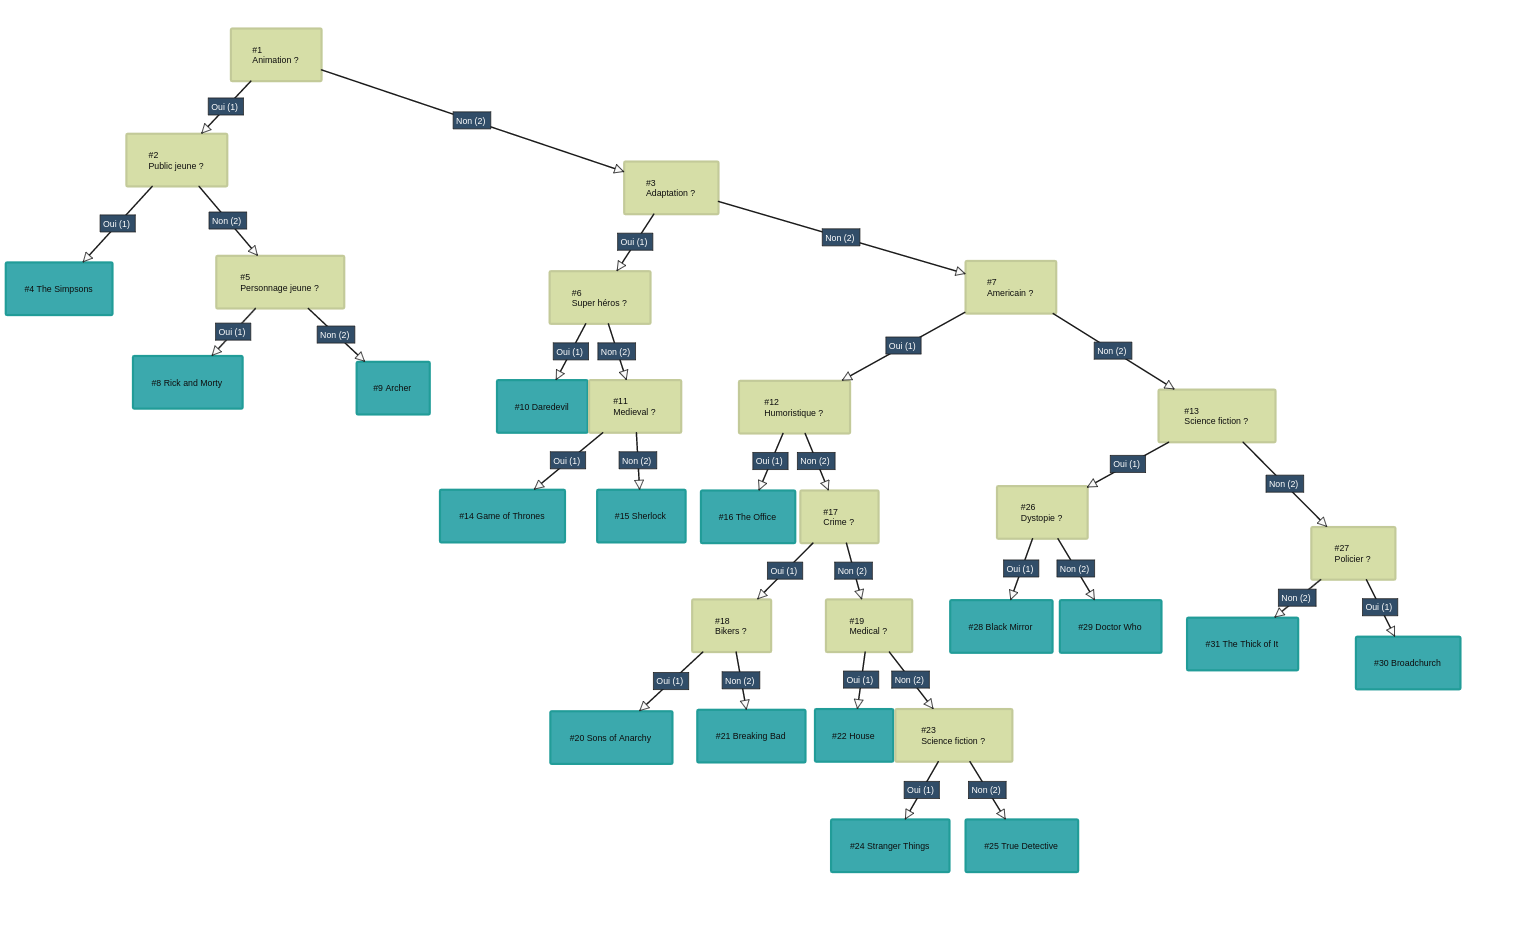
\includegraphics[scale=0.2]{arbre.png}
\caption{Arbre de décision}
\end{figure}
\end{frame}

\begin{frame}
\frametitle{Un système expert}
\framesubtitle{Arbre de décision}
\begin{figure}
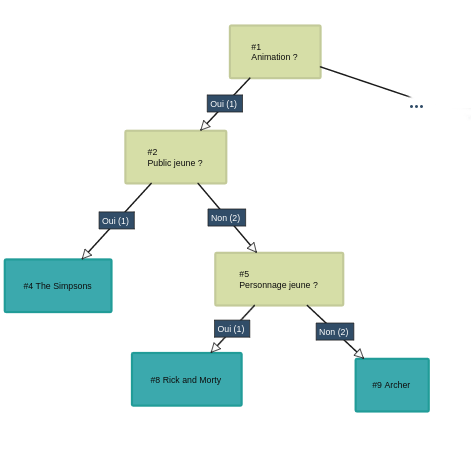
\includegraphics[scale=0.3]{arbre_zoom.png}
\caption{Zoom sur la branche animation de l'arbre de décision}
\end{figure}
\end{frame}

\begin{frame}
\frametitle{Caractéristiques du système final}
\begin{block}{Capacités}
\begin{itemize}
\item Interactif
\begin{itemize}
\item Oui (o.)
\item Non (n.)
\item Passe (p.)
\end{itemize}
\item Capacités de déductions
\item Régime par tentatives
\item Trois niveaux d'inférence
\item Capacités d'explications
\end{itemize}
\end{block}
\end{frame}

\begin{frame}
\begin{figure}
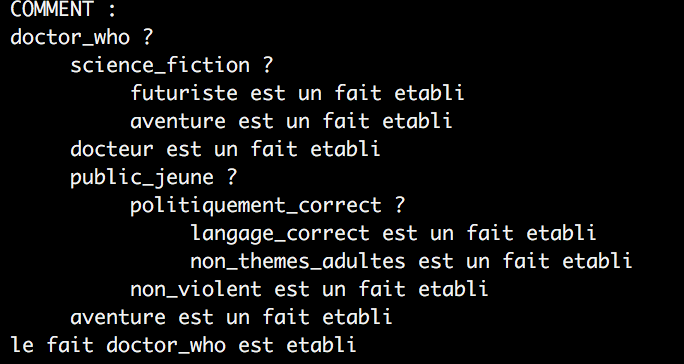
\includegraphics[scale=0.4]{exemple.png}
\caption{Le système déduit que la série recherchée est Doctor Who}
\end{figure}

\end{frame}

\end{document}